% CVPR 2023 Paper Template
% based on the CVPR template provided by Ming-Ming Cheng (https://github.com/MCG-NKU/CVPR_Template)
% modified and extended by Stefan Roth (stefan.roth@NOSPAMtu-darmstadt.de)

\documentclass[10pt,twocolumn,letterpaper]{article}

%%%%%%%%% PAPER TYPE  - PLEASE UPDATE FOR FINAL VERSION
\usepackage{cvpr}      % To produce the REVIEW version

% Include other packages here, before hyperref.
\usepackage{graphicx}
\usepackage{amsmath}
\usepackage{amssymb}
\usepackage{booktabs}
\usepackage{caption}
\usepackage{subcaption}
\usepackage{adjustbox}


% It is strongly recommended to use hyperref, especially for the review version.
% hyperref with option pagebackref eases the reviewers' job.
% Please disable hyperref *only* if you encounter grave issues, e.g. with the
% file validation for the camera-ready version.
%
% If you comment hyperref and then uncomment it, you should delete
% ReviewTempalte.aux before re-running LaTeX.
% (Or just hit 'q' on the first LaTeX run, let it finish, and you
%  should be clear).
\usepackage[pagebackref,breaklinks,colorlinks]{hyperref}

% Support for easy cross-referencing
\usepackage[capitalize]{cleveref}
\crefname{section}{Sec.}{Secs.}
\Crefname{section}{Section}{Sections}
\Crefname{table}{Table}{Tables}
\crefname{table}{Tab.}{Tabs.}

%%%%%%%%% PAPER ID  - PLEASE UPDATE
\def\cvprPaperID{*****} % *** Enter the CVPR Paper ID here
\def\confName{CVPR}
\def\confYear{2023}

\begin{document}

\newcommand{\dhimitrios}[1]{\textcolor{red}{Dhimitrios: #1}}

%%%%%%%%% TITLE - PLEASE UPDATE
\title{Team \#16: From Strings to Sequences --- Classifying and Generating Music from Acoustic Guitar Notes}


\author{
    Camilo Martínez\\
    7057573\\
    \and
    Dhimitrios Duka\\
    7059153\\
    \and
    Honglu Ma\\
    7055053\\
}
\maketitle

%%%%%%%%% BODY TEXT
\section{Abstract}
% Should be inside \emph{} https://openaccess.thecvf.com/content/CVPR2022W/WMF/papers/Guarnera_On_the_Exploitation_of_Deepfake_Model_Recognition_CVPRW_2022_paper.pdf
\emph{Lorem ipsum dolor sit amet, consectetur adipiscing elit}

\dhimitrios{We did not pre-train on EgoHands}

\section{Introduction}
Automatic chord recognition (ACR) is an information retrieval task that automatically recognizes the chords played in a music piece, whether it be an audio or video file. The ability to accurately recognize and identify chords is crucial for various downstream applications such as music analysis, music transcription, or even restoration of corrupted musical performances.

Our work aims to improve ACR in the context of acoustic guitars. We base our work on the previous work by \cite{Kristian_Zaman_Tenoyo_Jodhinata_2024} and extend it by exploring the potential of using state-of-the-art deep learning models and techniques while also adding an audio generation module at the end. Specifically, we investigate the feasibility of using the models from the YOLO \cite{redmon2016you} family and Faster R-CNN \cite{ren2016faster} for fretboard\footnote{The neck of the guitar.} recognition, alongside Vision Transformers \cite{dosovitskiy2020image} and DINOv2 \cite{oquab2023dinov2} for chord recognition. Additionally, we extend this work by implementing a chord-to-audio generation module, enabling the generation of audio directly from recognized chord labels.

\section{Related Work}
Over recent decades, many different approaches have been proposed to tackle the ACR task. The first ACR system was introduced in the late 1999s by \cite{takuya1999realtime}, where LISP music was utilized to perform chord recognition at the signal level. Since then, many signal-level-based approaches have been introduced ranging from chromagram-based method \cite{stark2009real}, to deep chromagram extractors \cite{korzeniowski2016feature}, to spectrogram-based feature extraction methods utilizing recurrent neural networks \cite{boulanger2013audio}. However, due to the inherent shortcomings of the aural approach in handling highly timbre sounds \cite{du2023conditional}, improvements plateaued.

With the rise of Computer Vision, researchers began exploring the potential of visual-based approaches to tackle the ACR task making use of hand patterns to perform chord classification. This approach was heavily based on the fact that humans often find it easier to recognize chords based on visual cues rather than auditory ones. \cite{su2020audeo} was able to successfully classify the chords being played on a piano and later on produce sound out of that information. Furthermore, \cite{tran2019cnn} and \cite{ooaku2018guitar} tried to replicate the same idea but applied to acoustic guitars. Even though both works used different techniques, the overall pipeline was the same. First, a model would be responsible for detecting the fretting hand within the image, cropping the image, and passing it through a classifier to determine the chord being played. However, this approach ignored the valuable information that could be retrieved from the fretboard itself.

Inspired by \cite{tran2019cnn, ooaku2018guitar}, \cite{Kristian_Zaman_Tenoyo_Jodhinata_2024} employed a Single Shot Detection (SSD) model \cite{sandler2018mobilenetv2}, pre-trained on the EgoHands \cite{Bambach_2015_ICCV} and ImageNet \cite{deng2009imagenet}. In contrast to previous works, they used the entire fretboard as input to the model, allowing it to learn the spatial relationships between the chords and frets achieving SOTA performance.

\section{Datasets}
We identified a significant gap in available datasets for the task of guitar chord recognition, which made us create our own. We recorded 90-second videos for each chord in three different environments, ensuring high quality by capturing them in 4K resolution at 60 frames per second. We extracted the frames from the video and downsampled them to a resolution of 640 $\times$ 360 pixels. This process generated approximately 30,000 frames per chord. To increase the diversity of the dataset, we used two different sampling methods: simple random sampling and KNN-based sampling. In the former method, we selected 1,000 frames at random, while in the latter, we used the KNN to choose the 1,000 frames that were the most distinct from one another.

\begin{figure}[h]
    \centering
    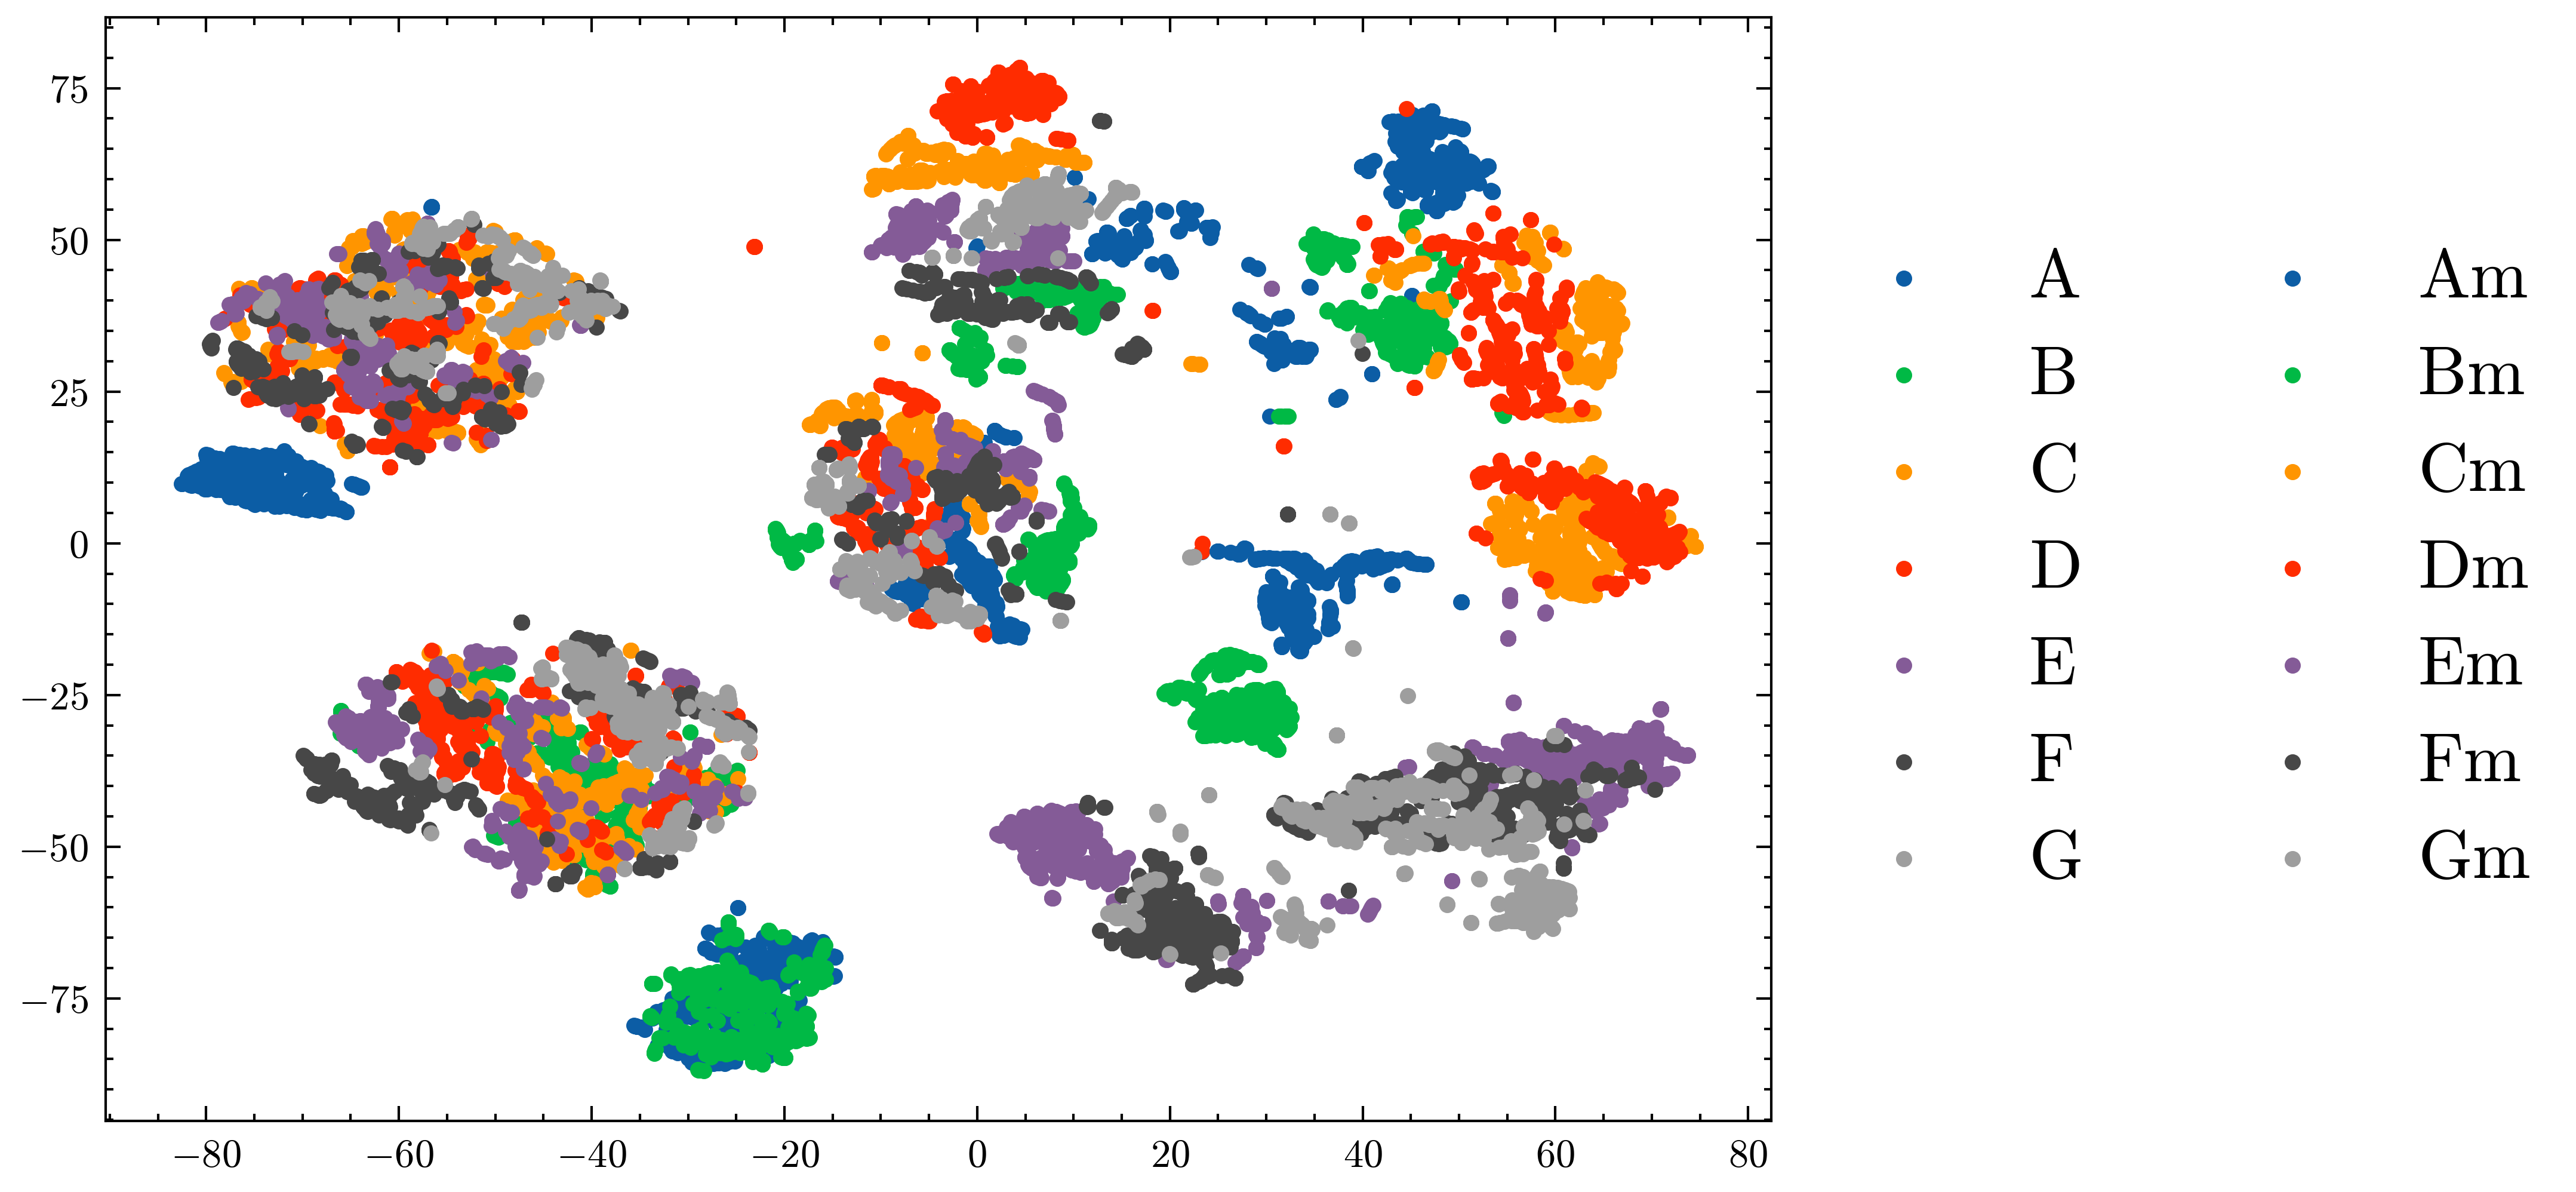
\includegraphics[width=0.48\textwidth]{images/final/Guitar-chords-ours_t-sne_plot.png}
    \caption{The t-SNE plot of our dataset containing 14 chords. Each point represents a KNN-sampled frame, with the color indicating the corresponding chord label.}
    \label{fig:ours-tsne-plot}
\end{figure}

Unfortunately, both sampling strategies resulted in an overly simplistic dataset that failed to capture the real-world complexity of chords, as shown by Figure \ref{fig:ours-tsne-plot}. This resulted in poor model generalization. However, rather than abandoning our dataset we used it as a test set to evaluate the generalizability of our model. In the end, we decided to use existing datasets \cite{guitar-chord-tvon8_dataset,guitar-chord-bounding-box_dataset, guitar-chord-handshape_dataset, guitar-chords-daewp_dataset} for training the models, merging them to create a more complex dataset which resulted in significantly better results.

This change in our approach necessitated a change in the scope of our chord recognition task. As a consequence of using existing datasets, we were limited to only seven chords in total—A, B, C, D, E, F, and G—down from the 14 chords originally planned.

\section{Methods}
In the following sections, we will give a overview of the methods used in our work for performing fretboard detection and guitar chord classification.

\subsection{Fretboard Detection}
For the freatboard detection task, we experimented with different models from the YOLO family and Faster R-CNN. We tried two different fine-tuning methods: freezing every layer except the last one and not freezing any layer, that is, finetuning the whole model. Both methods are fundamentally different and serve different purposes. The first method is used to finetune the model to a specific task while keeping the backbone as it is. This allows us to keep the previous learned features and classes. On the other hand, the second method will finetune the
whole model to the new task, while forgetting some of the previous learned features and classes. That is, the latter will have 2 classes after finetuning, the fretboard and the background.

\dhimitrios{Do we need to add more here?}

\subsection{Guitar Chord Classification}

\subsubsection{Hand Pose Estimation + Classifier}
First, we wanted to try a simple yet interesting approach. For a given sample image, we utilized a hand pose estimation model to extract the hand shape from it, which was then used as the input to a classifier.

\begin{figure}[h]
    \centering
    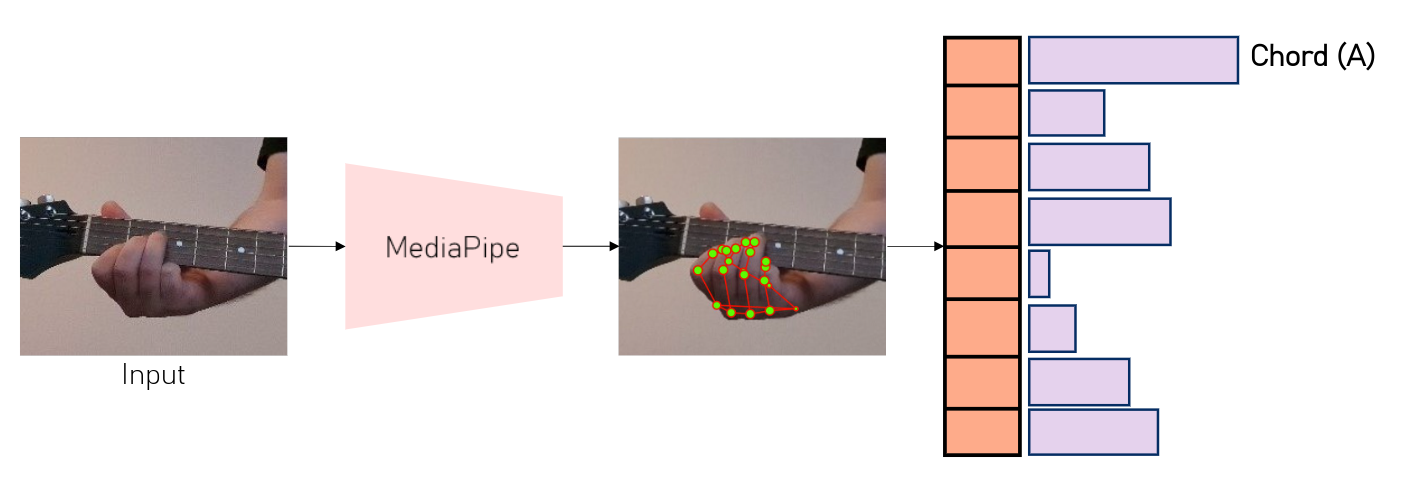
\includegraphics[width=0.5\textwidth]{images/final/hand_pose_estimation_classifier.png}
    \caption{The pipeline of the Hand Pose Estimation + Classifier approach. First, the image is passed through a hand pose estimation model to extract the landmarks. Then the result is passed through a classifier to determine the chord being played.}
    \label{fig:hand-pose-estimation-classifier}
\end{figure}

We used MediaPipe to extract the hand shape followed by different classifiers—SVM \cite{cortes1995support}, Random Forest \cite{ho1995random}, and a simple MLP—to classify the chords.

\subsubsection{Classifier only approach}
Next, we wanted to explore the potential benefits of using more advanced architectures to perform chord classification. We decided to experiment with Vision Transformers (ViT) \cite{dosovitskiy2020image}, specifically ViT-B/16, ViT-B/32, ViT-L/16, and ViT-L/32, to assess how different configurations of patch sizes and model sizes would impact performance. Additionally, we were also interested in evaluating the effectiveness of pre-trained self-supervised models in our task, so we also included DINOv2 \cite{oquab2023dinov2} in our experiments. This allowed us to compare their performance against the ViT models and explore whether self-supervised learning offers advantages in this task.

\section{Experimental Results and Analyses}
\label{sec:results}

In the following sections, we will present the results of our experiments and provide an analysis of the performance of the models used in our work.

\subsection{Fretboard Detection}

\begin{table}[thb]
    \scriptsize
    \centering
    \begin{tabular}{lcccc}
        \toprule
        \textbf{Model}          & \textbf{P} & \textbf{R} & \textbf{mAP50-95} & \textbf{mAP50} \\
        \midrule
        YOLOv8                  & 98.0\%     & 93.6\%     & 88.7\%            & 97.4\%         \\
        YOLOv9                  & 95.6\%     & 92.2\%     & 82.3\%            & 96.1\%         \\
        YOLOv10                 & 89.4\%     & 85.2\%     & 76.1\%            & 92.2\%         \\
        YOLOv8 (FB)             & 84.0\%     & 82.5\%     & 68.5\%            & 88.7\%         \\
        YOLOv9 (FB)             & 84.0\%     & 82.5\%     & 77.2\%            & 94.1\%         \\
        YOLOv10 (FB)            & 80.8\%     & 80.2\%     & 71.2\%            & 93.0\%         \\
        Faster-RCNN-Resnet50         & 80.5\%     & 79.9\%     & 77.6\%            & 93.9\%         \\
        Faster-RCNN-Resnet50 (FB)    & 61.4\%     & 65.4\%     & 52.2\%            & 85.6\%         \\
        Faster-RCNN-MobileNetv3      & 68.9\%     & 71.1\%     & 57.8\%            & 86.1\%         \\
        Faster-RCNN-MobileNetv3 (FB) & 76.9\%     & 74.6\%     & 65.7\%            & 93.0\%         \\
        \bottomrule
    \end{tabular}
    \caption{Performance metrics of different models on the evaluation dataset, shown in percentages. Each column represents a specific metric: Precision, Recall, mAP50-95, and mAP50. (FB) denotes models finetuned with a Frozen Backbone.}
    \label{tab:metrics-results}
\end{table}



\begin{figure}[thb]
    \centering
    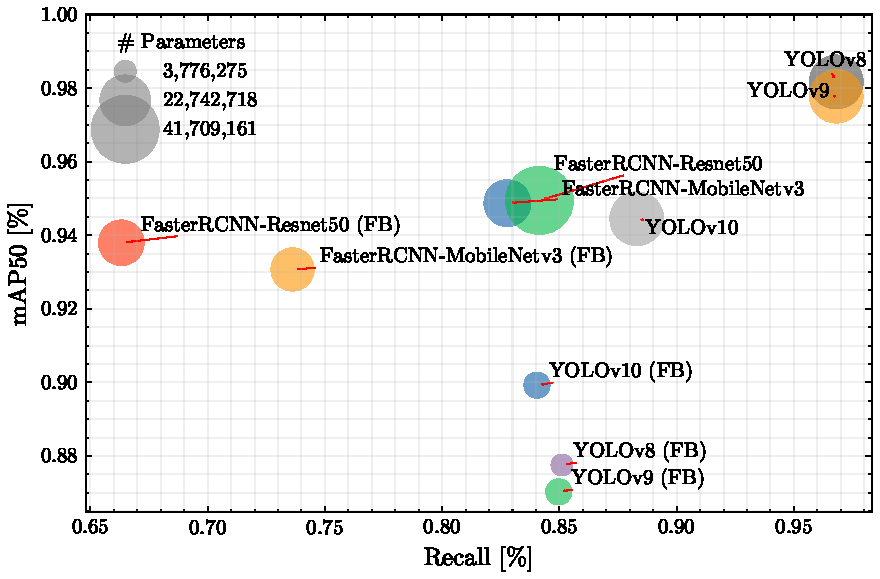
\includegraphics[width=\columnwidth]{images/final/recall_vs_map50.pdf}
    \caption{Recall vs. mAP@50 for the models tested and finetuned on the \emph{fretboard} class.}
    \label{fig:fretboard-models-recall-map}
\end{figure}

Since our YOLOv9 model did not lose its capability to detect the original 80 classes from the COCO dataset \cite{lin2015microsoftcococommonobjects}, we decided to re-evaluate its performance on the whole COCO dataset to quantify how much the finetuning process affected the original pre-trained model's performance. The results are shown in Figure \ref{fig:yolo-diff-confusion-matrix}, which shows a subset\footnote{We are only showing a subset of the classes for better visualization and space contraints.} of the confusion matrix of our model, and in Table \ref{tab:confusion-matrix-results}, where positive values are desirable for diagonal entries (indicating correct classifications), and negative values are preferred for off-diagonal entries (indicating reduced misclassifications).

\begin{figure}[h]
    \centering
    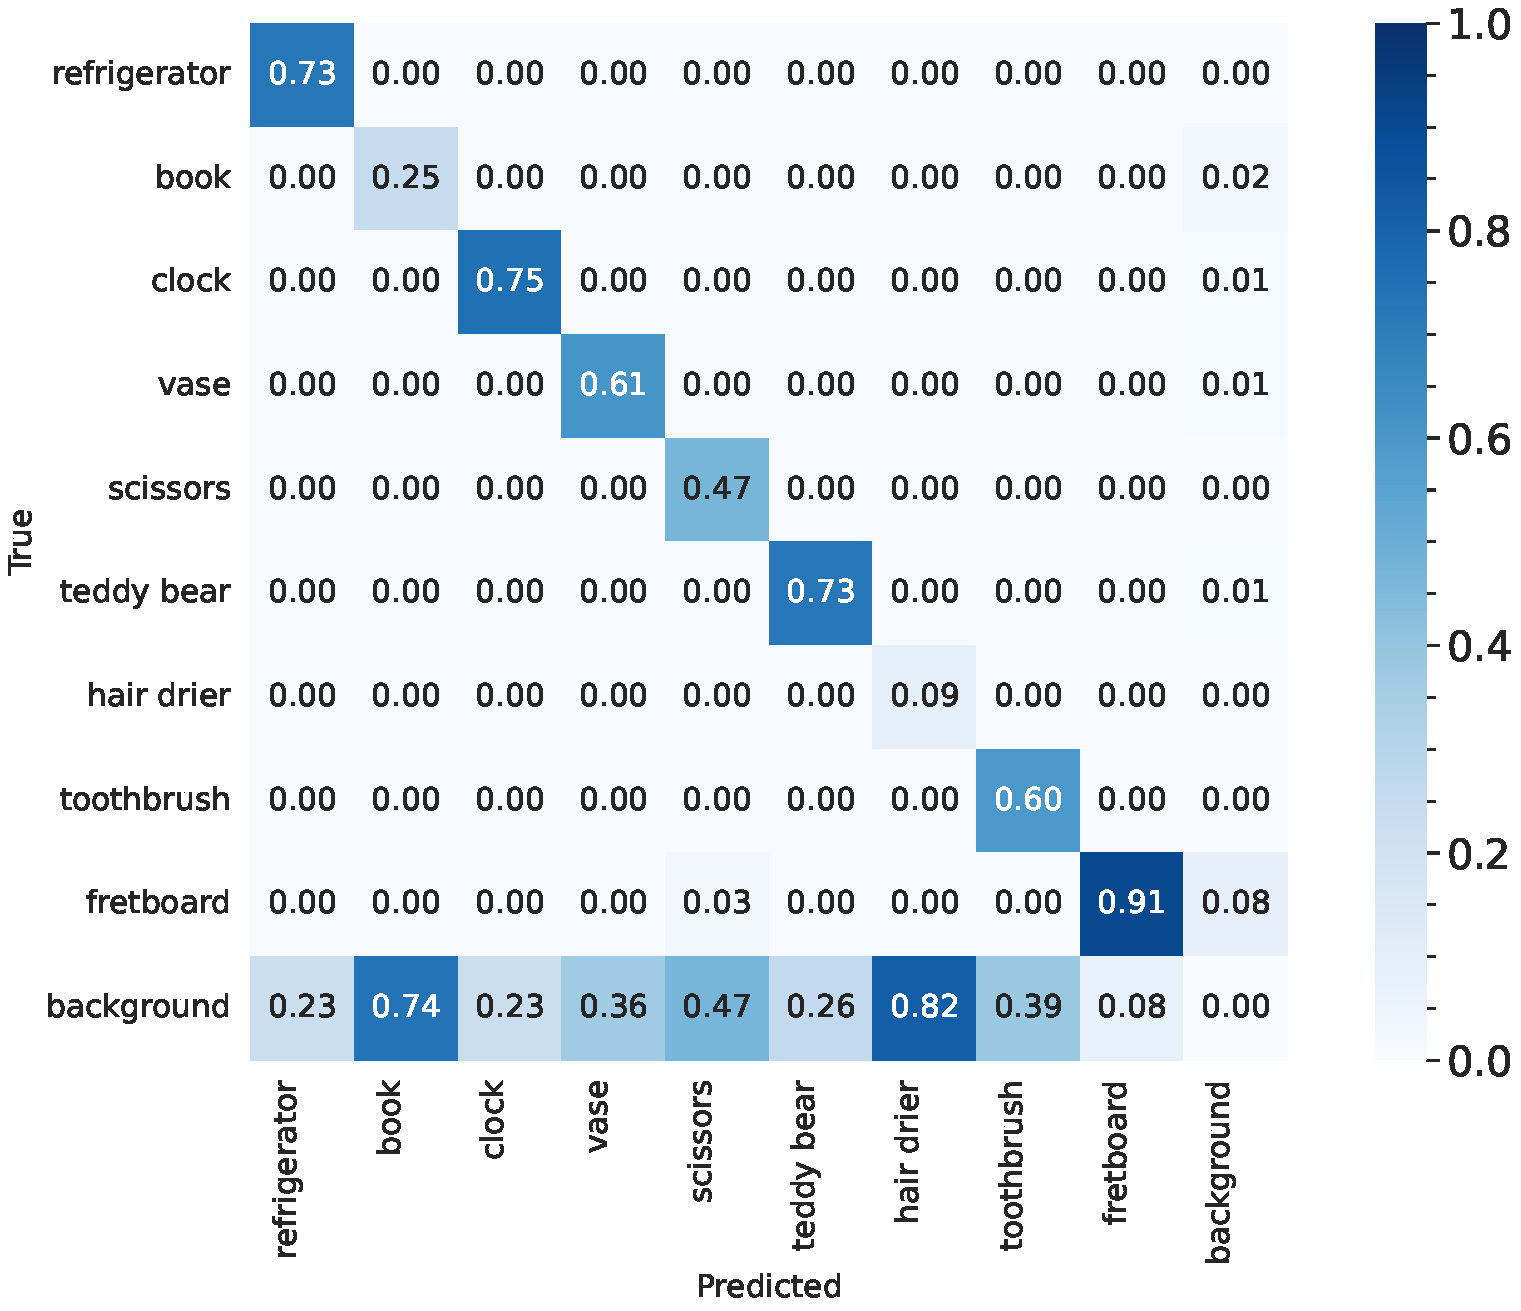
\includegraphics[width=0.5\textwidth]{images/final/yolo_confusion_matrix_subset.pdf}
    \caption{Confusion matrix of the YOLOv9 model on a subset of 10 classes from the original COCO dataset \cite{lin2015microsoftcococommonobjects}, plus our \emph{fretboard} class.}
    \label{fig:yolo-diff-confusion-matrix}
\end{figure}

\begin{table}[h]
    \centering
    \begin{tabular}{lcc}
        \toprule
        \textbf{Confusion Matrix Pos.} & \textbf{Positive} & \textbf{Negative} \\
        \midrule
        Diagonal                       & 1.41\%            & 5.38\%            \\
        \midrule
        Off-diagonal                   & 4.10\%            & 21.11\%           \\
        \bottomrule
    \end{tabular}
    \caption{Absolute sums of values (as \%) after taking the element-wise difference between the final confusion matrix obtained after finetuning the YOLOv9 model for our \emph{fretboard} class and the original confusion matrix of the pre-trained version on the COCO dataset. These values mean that, for the diagonal entries where the difference was positive, the model improved by 1.41\%, while for the off-diagonal entries where the difference was negative, the model improved by 21.11\%.}
    \label{tab:confusion-matrix-results}
\end{table}



\subsection{Guitar Chord Classification}
To evaluate our approaches against those in the original paper, we implemented the InceptionResNetv2 model as described by the authors. After training the model using the hyperparameters provided by \cite{Kristian_Zaman_Tenoyo_Jodhinata_2024} on our dataset, we obtained the results shown in Table \ref{tab:handpose-classifier-results}, which provided us with a baseline to compare our models against.

\begin{figure}[h]
    \centering
    \begin{subfigure}[t]{0.5\textwidth}
        \centering
        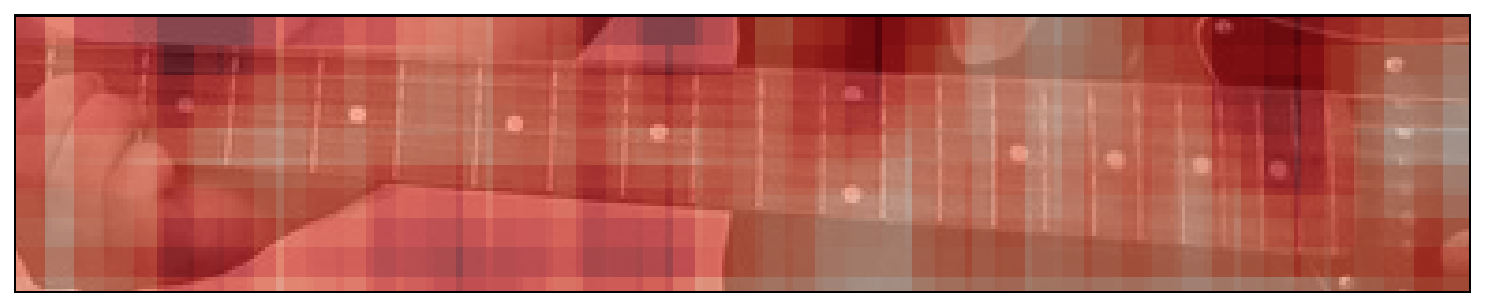
\includegraphics[width=\textwidth]{images/final/occlusion_untrained.pdf}
    \end{subfigure}
    \begin{subfigure}[t]{0.5\textwidth}
        \centering
        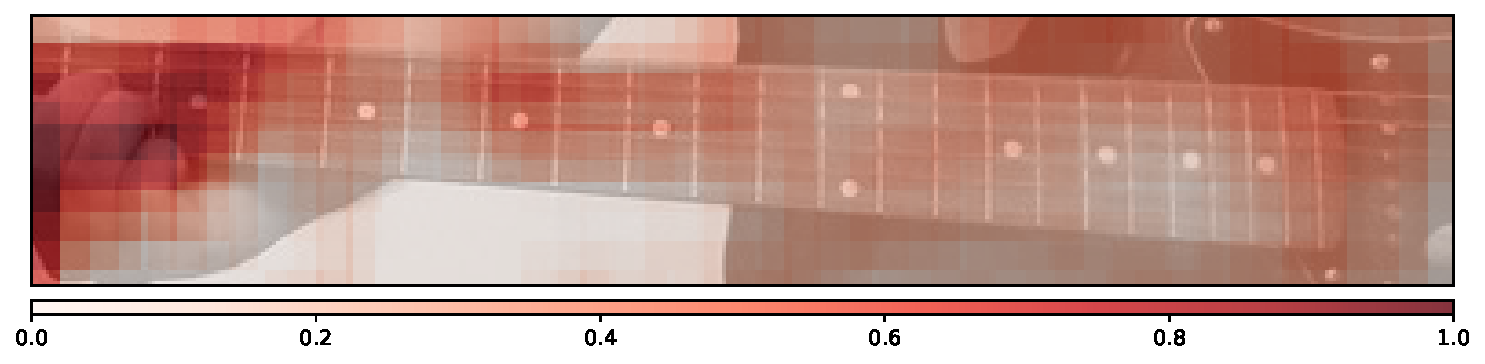
\includegraphics[width=\textwidth]{images/final/occlusion_trained.pdf}
    \end{subfigure}
    \caption{Occlusion-based attribution \cite{kokhlikyan2020captum} for model interpretability on a 74 $\times$ 389 input image using a stride of 8 and a sliding window of 30 $\times$ 30. \textbf{Top}: Untrained DINOv2 model. \textbf{Bottom}: Our DINOv2 model.}
    \label{fig:chord-classifier-visualization-fretboard}
\end{figure}

\begin{figure}[h]
    \centering
    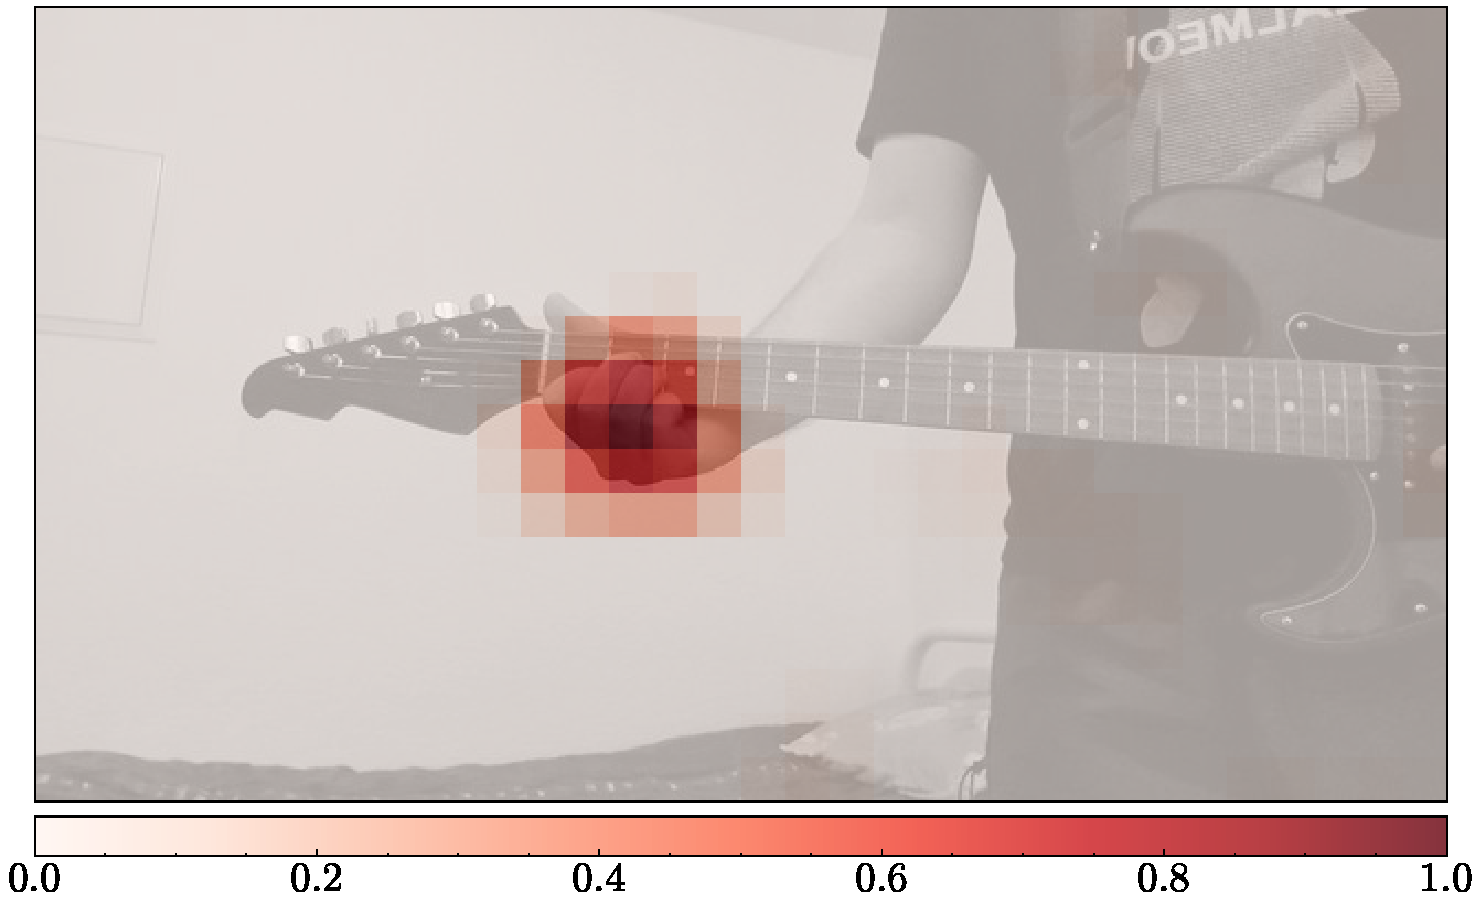
\includegraphics[width=0.5\textwidth]{images/final/occlusion_trained_full.pdf}
    \caption{Our DINOv2 model on a 360x640 input image using a stride of 20 and a sliding window of 60x60.}
    \label{fig:chord-classifier-visualization-fretboard-2}
\end{figure}

\subsubsection{Hand Pose Estimation + Classifier}
Surprisingly, this approach performed well, achieving good accuracy during validation and testing on two datasets. However, the model struggled to generalize to the third dataset, which was created by us. This outcome was anticipated, as the samples in our dataset were out of the training distribution, and the model lacked the complexity needed to generalize effectively to such data.

\begin{table}[h]
    \centering
    \begin{tabular}{lccc}
        \toprule
        \textbf{Model}    & \textbf{GC} & \textbf{GCT} & \textbf{GCO} \\
        \midrule
        InceptionResNetv2 & 83.56\%     & 68.63\%      & 15.57\%      \\
        \midrule
        SVM               & 95.27\%     & 85.71\%      & 18.61\%      \\
        Random Forest     & 93.35\%     & 52.41\%      & 16.16\%      \\
        MLP               & 89.44\%     & 78.57\%      & 14.39\%      \\
        \bottomrule
    \end{tabular}
    \caption{Accuracy of the Hand Pose Estimation + Classifier in the test set of different datasets. The following parameters where used: \texttt{SVM (C = 300)}, \texttt{Random Forest (n\_estimators = 200)}, and \texttt{MLP (hidden\_layer\_sizes = (100, 256, 100))}. Datasets used: \textbf{GC}: Guitar\_Chords, \textbf{GCT}: Guitar\_Chords\_Tiny, \textbf{GCO}: Guitar\_Chords\_Ours.}
    \label{tab:handpose-classifier-results}
\end{table}

\subsubsection{Classifier only approach}
To address this limitation of the previous approach, we decided to explore more complex models, such as Vision Transformers (ViT) and DINOv2. The results of our experiments are summarized in Table \ref{tab:transformer-models-results}.

\begin{table}[h]
    \centering
    \begin{tabular}{lccc}
        \toprule
        \textbf{Model}    & \textbf{GC} & \textbf{GCT} & \textbf{GCO} \\
        \midrule
        InceptionResNetv2 & 83.56\%     & 68.63\%      & 15.57\%      \\
        \midrule
        ViT-B/16          & \textbf{98.96} \%     & 85.29\%      & 96.24\%      \\
        ViT-B/32          & 93.07\%     & 81.37\%      & 95.83\%      \\
        ViT-L/16          & 95.84\%     & 81.37\%      & 12.29\%      \\
        ViT-L/32          & 77.03\%     & 43.14\%      & 13.43\%      \\
        DINOv2-S          & 96.24\%     & 88.24\%      & \textbf{98.18} \%      \\
        DINOv2-L          & 96.44\%     & \textbf{91.18}\%      & 97.92\%      \\
        \bottomrule
    \end{tabular}
    \caption{Accuracy of Classifier only apporach in the test set of different datasets.}
    \label{tab:transformer-models-results}
\end{table}

ViT models show varying performance across different datasets. The base models perform exceptionally well, with high accuracy on all datasets. However, the larger models do not exhibit the same performance. We argue that this is happening because the available is not sufficient to train large models effectively. Additionally, we can also observe that the patch 16 versions of the ViT models perform better than the patch 32 versions. This is likely due to the fact that the patch 16 versions have a higher resolution, which is important for accurately distinguishing between different hand positions.

Moreover, both DINOv2 variants, demonstrated strong and consistent performance across all datasets. The DINOv2-L model, in particular, achieved the highest accuracy on the \textbf{Guitar\_Chords\_Ours} dataset, slightly outperforming the small variant. The superior performance of DINOv2 can be attributed to its self-supervised learning approach. Unlike models pre-trained on ImageNet, which does not contain specific classes related to \emph{hands,} DINOv2's self-supervised learning allows it to develop more generic and transferable representations, leading to better generalization in our specific task. This enhanced generalization is further supported by attention visualizations of the model when applied to images from \textbf{Guitar\_Chords\_Ours} dataset, where the model correctly focuses on the hand performing the fretting, Figure \ref{fig:chord-classifier-visualization-fretboard} and \ref{fig:chord-classifier-visualization-fretboard-2}. However, an interesting thing that we noticed is that the model, if complex enougg, can learn to attent to the freting hand whithout providing it with the croped version of the image containing only the freatboard. This is a very interesting result that we will further investigate in the future and in order to do so, more data is needed because currently most of the data is in a croped format not including the compled fretboard too.

\section{Conclusion}

\section{Discussion}
Currently, we are missing a background class in the dataset.


    %%%%%%%%% REFERENCES
    {\small
        \bibliographystyle{ieee_fullname}
        \bibliography{references}
    }

\end{document}